\documentclass[12pt,a4paper]{article}
\usepackage[utf8]{inputenc}
\usepackage[catalan]{babel}
\usepackage{graphicx}
\usepackage{geometry}
\usepackage{fancyhdr}
\usepackage{tabularx}
\usepackage{lastpage}
\usepackage{enumitem}
\usepackage{amsmath}
\usepackage{amsfonts}
\usepackage{tikz} 
\usepackage{xcolor} 
\usepackage{mdframed} % Per als requadres d'exemples
\usetikzlibrary{calc}

% 1. MARGES I CAPÇALERA
\geometry{top=3cm, bottom=3cm, left=2cm, right=2cm, headheight=2cm}

\pagestyle{fancy}
\fancyhf{}
% Descomenta si tens logos
% \fancyhead[L]{
\includegraphics[height=1.5cm]{Logo_Departament.png}} 
% \fancyhead[R]{
\includegraphics[height=1.5cm]{Logo_Institut.png}}

\fancyfoot[L]{Departament de Matemàtiques}
\fancyfoot[C]{Pàgina \thepage\ de \pageref{LastPage}}
\fancyfoot[R]{}

\renewcommand{\headrulewidth}{0.4pt}

% Configuració de les llistes
\setlist[enumerate,1]{label=\textbf{\arabic*.}, leftmargin=*, itemsep=20pt}
\setlist[enumerate,2]{label=\alph*), leftmargin=*, itemsep=8pt}

% --- DEFINICIÓ DE CAIXES D'AJUDA I EXEMPLES ---

% Caixa per a exemples resolts
\newmdenv[
  backgroundcolor=gray!10,
  linecolor=black,
  linewidth=1pt,
  frametitle={Exemple resolt},
  frametitlerule=true,
  frametitlebackgroundcolor=gray!30,
  innertopmargin=10pt,
  innerbottommargin=10pt,
  roundcorner=5pt
]{exemple}

% Estil per a les pistes (text simple)
\newcommand{\pista}[1]{
    \par\vspace{2pt}
    {\small \color{blue!70!black} $\rightarrow$ \textit{\textbf{Pista:} #1}}
}

% Caixa per a fórmules o conceptes clau
\newcommand{\formulari}[1]{
    \begin{mdframed}[backgroundcolor=yellow!10, linecolor=orange, innerleftmargin=5pt, innerrightmargin=5pt]
        {\small #1}
    \end{mdframed}
}

\begin{document}

% --- PORTADA / CAPÇALERA ---
\begingroup
\renewcommand{\arraystretch}{2}
\begin{tabularx}{\textwidth}{|X|p{4cm}|}
    \hline
    \textbf{Nom i cognoms:} & \textbf{Grup:} \\ \hline
    \textbf{Activitat:} Dossier de Recuperació & \textbf{Data:} \\ \hline
\end{tabularx}
\endgroup

\vspace{0.5cm}
\begin{center}
    {\LARGE \textbf{RECUPERACIÓ DE MATEMÀTIQUES 3r ESO}} \\
    \vspace{0.2cm}
    {\large Dossier de treball i repàs}
\end{center}
\vspace{0.5cm}

% ==========================================
% BLOC 1: NUMÈRIC
% ==========================================
\section*{Bloc 1: Nombres Enters i Fraccions}

\begin{exemple}
\textbf{Operacions combinades:} Primer els parèntesis, després multiplicacions, al final sumes.
$$ 4 - 2 \cdot (-3) = 4 - (-6) = 4 + 6 = 10 $$
\textbf{Potències:} Atenció al signe!
$$ (-3)^2 = (-3)\cdot(-3) = +9 \quad \text{(Parell $\to$ Positiu)} $$
$$ (-2)^3 = (-2)\cdot(-2)\cdot(-2) = -8 \quad \text{(Senar $\to$ Negatiu)} $$
\end{exemple}

\begin{enumerate}
    \item \textbf{Operacions amb nombres enters.} Calcula pas a pas:
    \begin{enumerate}
        \item $-7 + 12 - 5 - 3 =$
        \item $(-8) \cdot (+3) =$
        \item $(-20) : (-4) =$
        \item $(-2)^3 =$ 
        \item $-3^2 =$ \pista{El signe menys està fora, no es multiplica per si mateix.}
        \item $15 - 3 \cdot [ 8 - (2 - 5) ] + (-2)^2 =$
    \end{enumerate}

\newpage
\begin{exemple}
\textbf{Simplificar fraccions:} Dividim dalt i baix pel mateix número.
$$ \dfrac{20}{30} = \dfrac{20 \div 10}{30 \div 10} = \dfrac{2}{3} $$ 
\textbf{Suma (MCM):} $$\frac{1}{2} + \frac{1}{3}.$$ $$ MCM(2,3)=6. $$  $$\frac{3}{6} + \frac{2}{6} = \frac{5}{6}$$
\textbf{Multiplicació (En línia):} $$\frac{2}{3} \cdot \frac{5}{7} = \frac{2\cdot5}{3\cdot7} = \frac{10}{21}$$.
\end{exemple}

    \item \textbf{Simplificació.} Simplifica fins a la fracció irreductible:
    \begin{enumerate}
        \item $\dfrac{24}{36} =$
        \item $\dfrac{45}{60} =$
    \end{enumerate}

    \item \textbf{Operacions amb fraccions.} 
    \begin{enumerate}
        \item $\dfrac{3}{4} - \dfrac{1}{6} + \dfrac{5}{3} =$ \vspace{0.2cm}
        \item $\dfrac{2}{5} \cdot \dfrac{10}{3} =$ \vspace{0.2cm}
        \item $\dfrac{7}{2} : \dfrac{3}{4} =$ \pista{Divisió: multiplica en creu (el caramel).} \vspace{0.2cm}
        \item $\dfrac{3}{2} - \dfrac{1}{4} \cdot \left( \dfrac{2}{3} + \dfrac{1}{6} \right) =$ 
    \end{enumerate}
\end{enumerate}

% ==========================================
% BLOC 2: PERCENTATGES (NOU)
% ==========================================
\newpage
\section*{Bloc 2: Percentatges i Vida Real}

\formulari{
    \textbf{Truc ràpid:} \\
    - Per calcular el \textbf{50\%} (la meitat), dividim per 2. \\
    - Per calcular el \textbf{10\%}, dividim per 10 (movem la coma un lloc). \\
    - Per calcular el \textbf{20\%}, calculem el 10\% i multipliquem per 2.
}

\begin{enumerate}[resume]
    \item \textbf{Test de conceptes.} Encercla la resposta correcta i explica per què l'has triat (sense fer càlculs complicats).
    
    \begin{enumerate}
        \item \textbf{El 20\% de 80 és...}
        \begin{itemize}
            \item[a)] 4
            \item[b)] 16
            \item[c)] 85
        \end{itemize}
        \textbf{Justificació:} \rule{10cm}{0.4pt}
        
        \item \textbf{Si em fan un descompte del 50\%, pagaré...}
        \begin{itemize}
            \item[a)] El doble
            \item[b)] La meitat
            \item[c)] El mateix
        \end{itemize}
        \textbf{Justificació:} \rule{10cm}{0.4pt}
    \end{enumerate}

    \item \textbf{Càlculs senzills.} Omple els buits:
    \begin{itemize}
        \item El 50\% de 200 € és \textbf{\dots\dots\dots €}
        \item El 10\% de 50 € és \textbf{\dots\dots\dots €}
        \item El 25\% (la quarta part) de 40 alumnes són \textbf{\dots\dots\dots alumnes.}
    \end{itemize}

    \item \textbf{Problemes reals.}
    \begin{enumerate}
        \item \textbf{Les Rebaixes:} Uns pantalons costen 40 €. Si tenen un descompte del 20\%, quants diners em descompten? Quant acabaré pagant?
        \vspace{2cm}
        
        \item \textbf{L'IVA:} Un videojoc costa 50 € sense IVA. Si li hem de sumar el 21\% d'IVA, quin serà el preu final?
        \pista{Calcula el 21\% de 50 (multiplica $50 \cdot 0,21$) i suma-ho al preu inicial.}
        \vspace{2cm}
    \end{enumerate}
\end{enumerate}

% ==========================================
% BLOC 3: POTÈNCIES I RADICALS
% ==========================================
\section*{Bloc 3: Notació Científica i Radicals}

\begin{exemple}
\textbf{Notació científica ($a \cdot 10^n$):}
\begin{itemize}
    \item $45.000 \to 4,5 \cdot 10^4$ (movem la coma 4 llocs a l'esquerra).
    \item $0,003 \to 3 \cdot 10^{-3}$ (movem la coma 3 llocs a la dreta $\to$ exponent negatiu).
\end{itemize}
\end{exemple}

\begin{enumerate}[resume]
    \item \textbf{Notació científica.} Escriu en la forma $a \cdot 10^n$:
    \begin{enumerate}
        \item $150.000.000 =$
        \item $0,000045 =$
        \item $3.200 =$
    \end{enumerate}

    \item \textbf{Pas a decimal.}
    \begin{enumerate}
        \item $2,5 \cdot 10^4 =$ 
        \item $1,2 \cdot 10^{-3} =$ 
    \end{enumerate}

\begin{exemple}
\textbf{Radicals:} Busquem l'origen de la potència.
\begin{itemize}
    \item $\sqrt{16} = 4$ perquè $4^2 = 16$.
    \item $\sqrt[3]{-27} = -3$ perquè $(-3) \cdot (-3) \cdot (-3) = -27$.
\end{itemize}
\end{exemple}

    \item \textbf{Radicals.} Calcula:
    \begin{enumerate}
        \item $\sqrt{49} =$
        \item $\sqrt{100} =$
        \item $\sqrt[3]{27} =$
        \item $\sqrt[3]{-8} =$
    \end{enumerate}
\end{enumerate}

% ==========================================
% BLOC 4: ÀLGEBRA
% ==========================================
\newpage
\section*{Bloc 4: Àlgebra i Polinomis}

\begin{exemple}
\textbf{Suma/Resta:} Ajuntem per famílies (les $x^2$ amb les $x^2$, els nombres amb nombres).
$$ (3x + 5) + (2x - 2) = 5x + 3 $$
\textbf{Multiplicació:} Nombre per tot el parèntesi.
$$ 2 \cdot (3x + 4) = 6x + 8 $$
\textbf{Identitat Notable $(a+b)^2$:} El primer al quadrat + 2 pel primer pel segon + el segon al quadrat.
$$ (x+3)^2 = x^2 + 2\cdot x \cdot 3 + 3^2 = x^2 + 6x + 9 $$
\end{exemple}

\begin{enumerate}[resume]
    \item \textbf{Operacions amb polinomis.} Donats $P(x) = 3x^2 - 2x + 5$ i $Q(x) = x^2 + 4x - 2$:
    \begin{enumerate}
        \item $x + x =$
        \item $x \cdot x =$
        \item $P(x) + Q(x) =$
        \item $P(x) - Q(x) =$ \pista{El menys canvia TOTS els signes de Q(x).}
        \item $x \cdot (2x + 3) =$
        \item $(x + 2) \cdot (x - 3) =$ \pista{Multiplica tots per tots (4 multiplicacions).}
    \end{enumerate}

    \item \textbf{Identitats notables.} Desenvolupa:
    \begin{enumerate}
        \item $(x + 3)^2 =$
        \item $(x - 4)^2 =$
        \item $(x + 5) \cdot (x - 5) =$
    \end{enumerate}
\end{enumerate}
\newpage
% ==========================================
% BLOC 5: EQUACIONS
% ==========================================
\section*{Bloc 5: Equacions}

\begin{exemple}
\textbf{Equació 1r grau:} Objectiu $\to$ deixar la $x$ sola.
$$ 4x - 2 = x + 7 $$
1. Passem les $x$ a l'esquerra i nombres a la dreta (canviant de signe):
$$ 4x - x = 7 + 2 $$
2. Operem:
$$ 3x = 9 $$
3. El 3 que multiplica passa dividint:
$$ x = \frac{9}{3} \rightarrow x = 3 $$
\end{exemple}

\begin{enumerate}[resume]
    \item \textbf{Equacions de primer grau.} 
    \begin{enumerate}
        \item $5x - 3 = 2x + 9$ \vspace{1.5cm}
        \item $3(x - 2) + 4 = 10$ \pista{Primer treu el parèntesi multiplicant.} \vspace{1.5cm}
        \item $\dfrac{x}{2} + \dfrac{x-1}{3} = 3$ \pista{Multiplica TOTA l'equació per 6 per eliminar fraccions.} \vspace{2cm}
    \end{enumerate}
\newpage
\begin{exemple}
\textbf{Equació 2n grau:} $ax^2 + bx + c = 0$.
Exemple: $x^2 - 3x + 2 = 0$. Aquí $a=1, b=-3, c=2$.
$$ x = \frac{-(-3) \pm \sqrt{(-3)^2 - 4\cdot1\cdot2}}{2\cdot1} = \frac{3 \pm \sqrt{9 - 8}}{2} = \frac{3 \pm 1}{2} $$
Solucions: $\frac{4}{2}=2$ i $\frac{2}{2}=1$.
\end{exemple}

    \item \textbf{Equació de segon grau.} Resol:
    \begin{enumerate}
        \item $x^2 - 5x + 6 = 0$ \vspace{3cm}
    \end{enumerate}

    \item \textbf{Problemes d'equacions.} Planteja i resol:
    \begin{enumerate}
        \item Troba un nombre que, si li sumes 12, dona com a resultat 35. \vspace{2cm}
        \item En una classe hi ha el doble de nois ($2x$) que de noies ($x$). Si en total són 27 alumnes, quants nois i quantes noies hi ha? \vspace{3cm}
    \end{enumerate}
\end{enumerate}

\newpage

% ==========================================
% BLOC 6: FUNCIONS
% ==========================================
\section*{Bloc 6: Funcions}

\begin{enumerate}[resume]
    \item \textbf{Taules de valors i representació.}
    \pista{Substitueix la $x$ a la fórmula. Exemple: Si $y=x+1$ i $x=2 \to y=2+1=3$.}
    
    \begin{enumerate}
        \item Completa la taula per a $y = 2x$ i per a $y = x + 3$.
        
        \begin{center}
        \begin{tabular}{|c|c|}
            \hline
            $x$ & $y = 2x$ \\ \hline
            -2 &  \\ \hline
            -1 &  \\ \hline
            0 &  \\ \hline
            1 &  \\ \hline
            2 &  \\ \hline
        \end{tabular}
        \hspace{2cm}
        \begin{tabular}{|c|c|}
            \hline
            $x$ & $y = x + 3$ \\ \hline
            -2 &  \\ \hline
            -1 &  \\ \hline
            0 &  \\ \hline
            1 &  \\ \hline
            2 &  \\ \hline
        \end{tabular}
        \end{center}

        \item Representa gràficament les dues funcions:
        \begin{center}
        \begin{tikzpicture}[scale=0.7]
            \draw[thin, lightgray] (-5,-5) grid (5,5);
            \draw[->, thick] (-5,0) -- (5,0) node[right] {$x$};
            \draw[->, thick] (0,-5) -- (0,5) node[above] {$y$};
            \foreach \x in {-4,-3,-2,-1,1,2,3,4} \draw (\x,1pt) -- (\x,-1pt) node[below] {\footnotesize \x};
            \foreach \y in {-4,-3,-2,-1,1,2,3,4} \draw (1pt,\y) -- (-1pt,\y) node[left] {\footnotesize \y};
        \end{tikzpicture}
        \end{center}
    \end{enumerate}

    \item \textbf{Problema de context.} El pes d'un camió buit és de 3.830 kg. Transporta sacs de 25 kg.
    \begin{enumerate}
        \item Escriu la fórmula de la funció ($y = \text{Pes Inicial} + \text{Pes per sac} \cdot x$).
        \item Quant pesarà el camió si porta 100 sacs?
    \end{enumerate}
\end{enumerate}
\newpage
% ==========================================
% BLOC 7: ESTADÍSTICA
% ==========================================
\section*{Bloc 7: Estadística}

\begin{enumerate}[resume]
    \item \textbf{Taula de freqüències.} 
    \pista{\textbf{Freq. Absoluta ($n_i$):} Compta quants cops surt cada número. \\ 
    \textbf{Freq. Relativa ($f_i$):} Divideix el recompte pel Total d'alumnes. \\
    \textbf{Percentatge (\%):} Multiplica la freq. relativa per 100.}
    
    Dades (Talla de peu): $38, 40, 39, 41, 42, 38, 40, 39, 39, 37, 40, 41, 39, 38, 40, 42, 39, 40, 37, 40$.
    \vspace{4cm}

    \item \textbf{Càlcul de paràmetres.}
    \begin{enumerate}
        \item Omple la taula següent (multiplica les columnes com s'indica a la capçalera):
        \begin{center}
        \begin{tabular}{|c|c|c|c|}
            \hline
            Alçada ($x$) & Alumnes ($n$) & Multiplica $x \cdot n$ & Multiplica $x^2 \cdot n$ \\ \hline
            160 & 4 & $160 \cdot 4 = 640$ & $160^2 \cdot 4 = 102.400$ \\ \hline
            165 & 6 & & \\ \hline
            170 & 8 & & \\ \hline
            175 & 5 & & \\ \hline
            180 & 2 & & \\ \hline
            \textbf{Total} & \textbf{25} & \textbf{Suma A =} & \textbf{Suma B =} \\ \hline
        \end{tabular}
        \end{center}
        
        \item \textbf{Mitjana:} Agafa el resultat de la \textbf{Suma A} i divideix-lo pel Total d'alumnes (25).
        \vspace{1cm}
        
        \item \textbf{Desviació típica:} Segueix la fórmula: $\sqrt{\dfrac{\text{Suma B}}{25} - (\text{Mitjana})^2}$
    \end{enumerate}
\end{enumerate}

\newpage

% ==========================================
% BLOC 8: GEOMETRIA
% ==========================================
\section*{Bloc 8: Geometria}

\begin{enumerate}[resume]
    \item \textbf{Teorema de Tales.} Les rectes $r$, $s$ i $t$ són paral·leles.
    \formulari{La proporció es manté: $\dfrac{\text{Part Esquerra}}{\text{Part Esquerra}} = \dfrac{\text{Part Dreta}}{\text{Part Dreta}}$}
    Calcula $x$:
    \begin{center}
        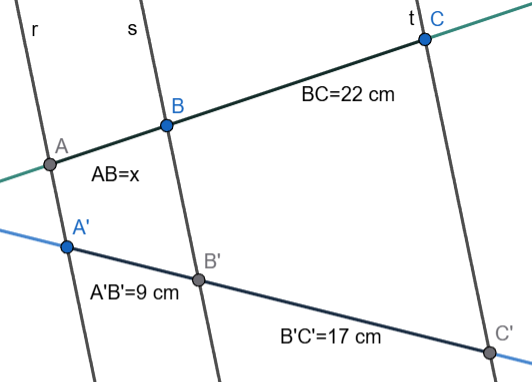
\includegraphics[width=0.6\textwidth]{ProblemaRectesParaleles.png}
    \end{center}

    \item \textbf{Semblança de triangles.}
    \formulari{Raó de semblança ($k$) = Quantes vegades és més gran el costat gran respecte al petit. \\ $k = \dfrac{\text{Costat Gran}}{\text{Costat Petit}}$}
    Determina $x$, $y$ i la raó de semblança.
    \begin{center}
        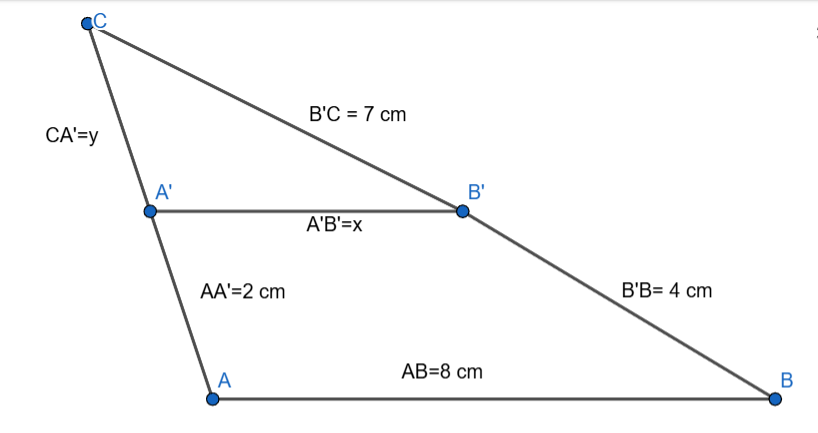
\includegraphics[width=0.6\textwidth]{ProblemaRaoSemblanca.png}
    \end{center}
\newpage
    \item \textbf{Teorema de Pitàgores.}
    \formulari{Sempre en triangles rectangles: $\text{Hipotenusa}^2 = \text{Catet}^2 + \text{Catet}^2$}
    \begin{enumerate}
        \item Catets de 6 cm i 8 cm. Quant mesura la hipotenusa?
        \item Una escala de 5 metres (hipotenusa) està recolzada a la paret. El peu és a 3 metres (catet). A quina alçada arriba (l'altre catet)?
        
        \begin{center}
        \begin{tikzpicture}[scale=0.5]
            \draw[thick] (0,0) -- (0,4) -- (3,0) -- cycle;
            \draw[dashed] (0,0) -- (3,0) node[midway, below] {$3\text{ m}$};
            \draw (1.5, 2.2) node[rotate=-53] {$5\text{ m}$};
            \node at (-0.5, 2) {$?$};
            \draw (0,0.3) -- (0.3,0.3) -- (0.3,0);
        \end{tikzpicture}
        \end{center}
    \end{enumerate}
\end{enumerate}

\end{document}